\documentclass[10pt]{hedlab}
\usepackage[utf8]{inputenc}
\usepackage[russian]{babel}
\usepackage[derivative,root]{hedmaths}
\usepackage{graphicx}

\usepackage{ucs}
\usepackage{listings}
\lstset{extendedchars=\true,inputencoding=utf8x,basicstyle=\footnotesize}
\usepackage[usenames,dvipsnames]{color}
\usepackage[colorlinks,linkcolor=black,citecolor=black,urlcolor=Blue]{hyperref}

\student{Чечеткин И. А.}
\date{04.03.2014}
\labname{Атом Томаса-Ферми}
\labnum{2}

\begin{document}
  \makeheader

  \section{Вывод уравнения Томаса-Ферми}

  Численные расчеты распределения заряда и поля в атоме методом
  самосогласованного поля чрезвычайно громоздки, в особенности для сложных
  атомов. Но как раз для сложных атомов существует другой приближенный метод,
  ценность которого заключается в его простоте; правда, он приводит к
  значительно менее точным результатам, чем метод самосогласованного поля. В
  основе этого метода лежит тот факт, что в сложных атомах с большим числом
  электронов большинство электронов обладает сравнительно большими главными
  квантовыми числами. В этих условиях применимо квазиклассическое приближение.
  Поэтому мы можем применить к состояниям отдельных электронов в атоме понятие
  о <<клетках в фазовом пространстве>>.

  Объем фазового пространства, соответствующий электронам, обладающим
  импульсом, меньшим чем \( p \), и находящимся в элементе объема \( dV \)
  физического пространства, равен \( (4 / 3)\pi p^3\,dV \). В соответствии с
  принципом неопределенности одно состояние в фазовом пространстве занимает
  объем \( (2\pi\hbar)^3 \) или \( (2\pi)^3 \) в атомных
  единицах\footnote{ Далее используются атомные единицы}. Этому объему
  соответствует \( (4 / 3)\pi p^3\,dV / (2\pi)^3 \) <<клеток>>, то есть
  возможных состояний, в которых может одновременно находиться не более
  \[
    2 \cdot \frac{4}{3}\frac{\pi p^3\,dV}{(2\pi)^3} = \frac{p^3\,dV}{3\pi^2}
  \]
  электронов (в одной <<клетке>> находятся два электрона с противоположными
  спинами). В нормальном состоянии атома электроны, находящиеся в каждом
  элементе объема \( dV \), должны заполнять клетки, соответствующие импульсу
  от нуля до некоторого максимального значения \( p_0 \), называемого
  импульсом Ферми. Тогда кинетическая энергия электронов будет иметь в каждой
  точке, вблизи которой находится объем \( dV \), по возможности меньшее
  значение. Если написать число электронов в объеме \( dV \), как
  \( n\cdot dV \) (где \( n \)~-- плотность числа электронов), то мы можем
  утверждать, что максимальное значение \( p_0 \) импульса электронов в каждой
  точке связано с \( n \) посредством соотношения
  \[
    n = \frac{p_0^3}{3\pi^2}.
  \]

  Максимальное же значение кинетической энергии электрона в месте, где
  электронная плотность есть \( n \), равно
  \begin{equation}
    \frac{p_0^2}{2} = \frac{1}{2} \Bigl(3\pi^2 n\Big)^{2 / 3}.
    \label{eq:1}
  \end{equation}

  Пусть \( \phi(r) \) есть электростатический потенциал, который мы принимаем
  равным нулю на бесконечности. Полная энергия электрона есть
  \( p^2 / 2 - \phi \). Очевидно, что полная энергия каждого электрона должна
  быть отрицательной; в противном случае электрон уйдет на бесконечность.
  Обозначим максимальное значение полной энергии электрона в каждой точке
  посредством \( -\phi_0 \), где \( \phi_0 \)~-- положительная постоянная.
  Таким образом, мы можем написать:
  \begin{equation}
    \frac{p_0^2}{2} = \phi - \phi_0.
    \label{eq:2}
  \end{equation}
  Приравнивая выражения \eqref{eq:1} и \eqref{eq:2}, получим
  \begin{equation}
    n = \left[ 2\bigl(\phi - \phi_0\big) \right]^{3 / 2} \frac{1}{3\pi^2}
    \label{eq:3}
  \end{equation}
  -- соотношение, связывающее электронную плотность и потенциал в каждой точке
  атома.

  При \( \phi = \phi_0 \) плотность \( n \) обращается в нуль; \( n \) должно
  быть положено равным нулю и во всей области, где \( \phi < \phi_0 \), и
  соотношение \eqref{eq:2} привело бы к отрицательной максимальной
  кинетической энергии. Таким образом, уравнением \( \phi = \phi_0 \)
  определяется граница атома. Но вне центрально-симметрического распределения
  зарядов с равным нулю полным зарядом поле отсутствует. Поэтому на границе
  нейтрального атома должно быть \( \phi = 0 \). Отсюда следует, что для
  нейтрального атома постоянная \( \phi_0 \) должна быть положена равной нулю.
  Напротив, для иона постоянная \( \phi_0 \) отлична от нуля\footnote{ Далее
  рассматривается нейтральный атом, поэтому \( \phi_0 \) полагается равным
  нулю}.

  Согласно электростатическому уравнению Пуассона, имеем \( \D\phi = 4\pi n \);
  подставляя сюда \eqref{eq:3}, получим основное уравнение Томаса-Ферми:
  \begin{equation}
    \D\phi = \frac{8\sqrt{2}}{3\pi}\phi^{3 / 2}.
    \label{eq:4}
  \end{equation}

  \section{Универсальная функция экранирования}

  Распределение поля в нормальном состоянии атома определяется
  центрально-симметричным решением этого уравнения, удовлетворяющим следующим
  граничным условиям: при \( r \to 0 \) поле должно переходить в кулоновское
  поле ядра, то есть должно быть \( \phi r \to Z \); при \( r \to \infty \)
  должно быть \( \phi r \to 0 \). Вводя вместо переменной \( r \) новую
  переменную \( x \), согласно определениям
  \begin{equation}
    r = xbZ^{-1 / 3}, \quad\text{где}\quad b = \frac{1}{2} \left(
      \frac{3\pi}{4} \right)^{2 / 3} = 0,\!885,
    \label{eq:5}
  \end{equation}
  а вместо \( \phi \) новую неизвестную функцию \( \Phi \):
  \begin{equation}
    \phi(r) = \frac{Z}{r} \Phi \left( \frac{rZ^{1 / 3}}{b} \right) =
      \frac{Z^{4 / 3}}{b} \frac{\Phi(x)}{x},
    \label{eq:6}
  \end{equation}
  в единицах СГС:
  \[
    \phi(r) = \frac{Ze}{r} \Phi \left( \frac{rZ^{1 / 3}}{0,\!885}r_B \right).
  \]
  Получим уравнение
  \begin{equation}
    x^{1 / 2} \dder{\Phi}{x} = \Phi^{3 / 2}
    \label{eq:7}
  \end{equation}
  с граничными условиями \( \Phi = 1 \) при \( x = 0 \) и \( \Phi = 0 \) при
  \( x = \infty \). Это уравнение не содержит уже никаких параметров и
  определяет универсальную функцию экранирования Томаса-Ферми \( \Phi(x) \).

  \section{Численное решение}
  \begin{figure}[h!]
    \vspace{-1em} \hspace{-2em}
      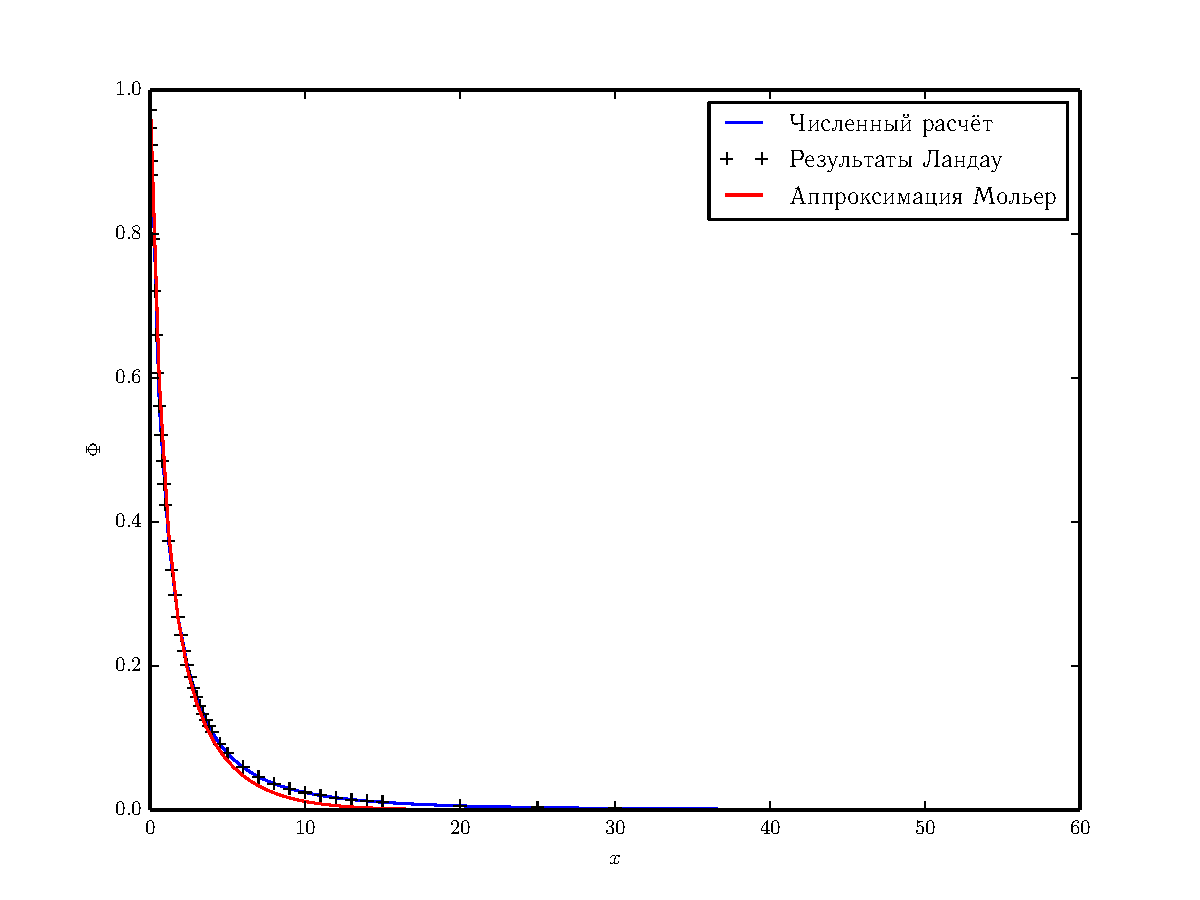
\includegraphics[width=.55\textwidth]{common} \hspace{-3em}
      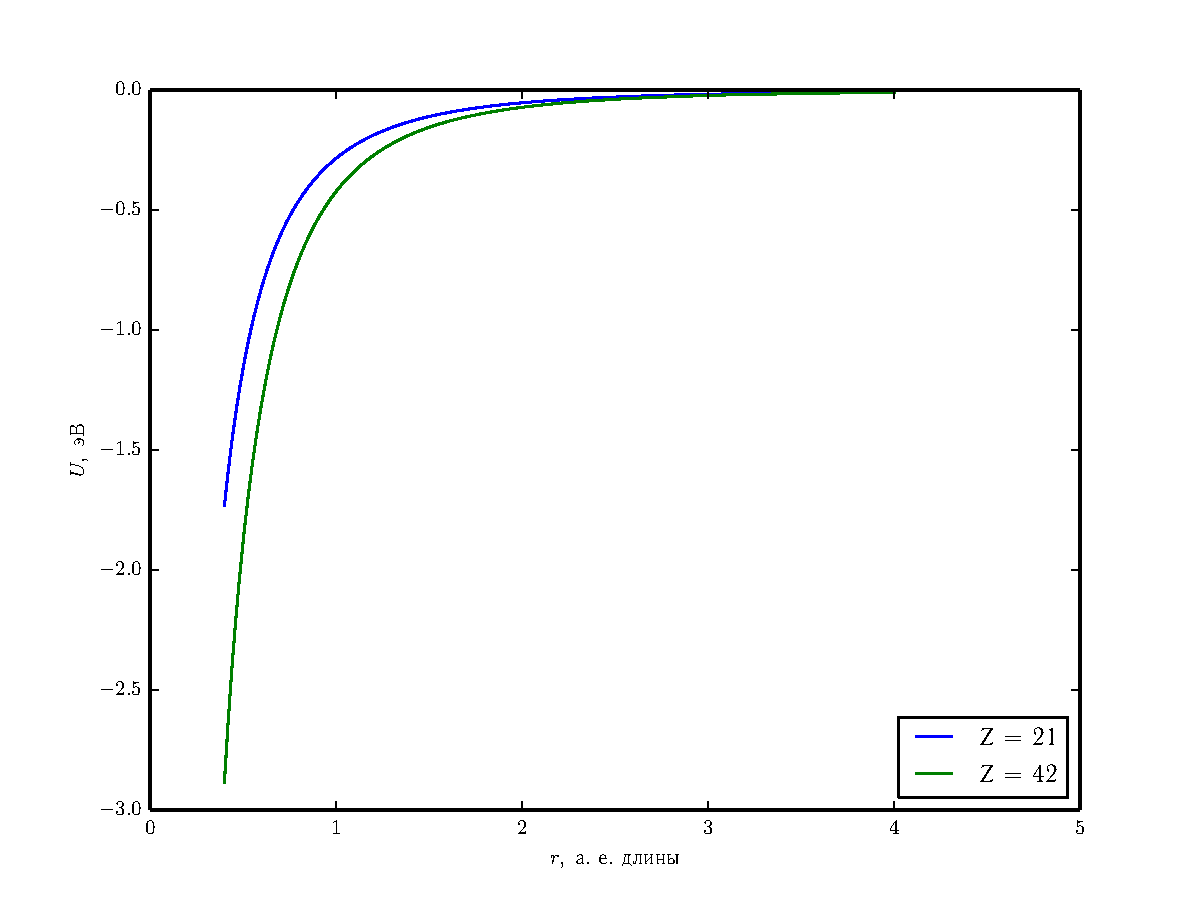
\includegraphics[width=.55\textwidth]{Z_21_42} \\
    \parbox{.49\textwidth}{\caption{Решение уравнения Томаса--Ферми
      \eqref{eq:7}} \label{fig:1}}
      \parbox{.49\textwidth}{\caption{Зависимость потенциальной энергии
      электрона \( U \) от координаты \( r \)} \label{fig:2}}    
  \end{figure}
  \newpage
  \section{Листинги программ}
  \lstinputlisting[language=c++,caption=Расчёт решения уравнения Томаса-Ферми]{code/lab2.cpp}
  \lstinputlisting[language=python,caption=Построение графиков]{code/lab2.py}
 
\end{document}
